\documentclass[11pt]{article}  % [12pt] option for the benefit of aging markers
\usepackage{amssymb,amsthm}    % amssymb package contains more mathematical symbols
\usepackage{graphicx}          % graphicx package enables you to paste in graphics
\usepackage[document]{ragged2e} 
\usepackage{float}
\usepackage{tabularx}
\usepackage{multirow}
\usepackage{setspace}

%%%%%%%%%%%%%%%%%%%%%%%%%%%%%%%%%
%
%    Page size commands.  Don't worry about these
%
\setlength\topmargin{0pt}
\addtolength\topmargin{-\headheight}
\addtolength\topmargin{-\headsep}
\setlength\oddsidemargin{0pt}
\setlength\textwidth{\paperwidth}
\addtolength\textwidth{-2in}
\setlength\textheight{\paperheight}
\addtolength\textheight{-2in}
\doublespacing

%%%%%%%%%%%%%%%%%%%%%%%%%%%%%%%%%%%%%%%%%%%%%%%%%%%%%%%%%%%%%%%
%
%    Definitions of environments for theorems etc.
%
\newtheorem{theorem}{Theorem}[section]          % Theorems numbered within sections - eg Theorem 2.1 in Section 2.
\newtheorem{corollary}[theorem]{Corollary}      % Corollaries etc. will be counted as Theorems for numbering
\newtheorem{lemma}[theorem]{Lemma}              % eg Lemma 3.1, ... Theorem 3.2, ... Corollary 3.3.
\newtheorem{proposition}[theorem]{Proposition}
\newtheorem{conjecture}[theorem]{Conjecture}

\theoremstyle{definition}
\newtheorem{definition}[theorem]{Definition}

\theoremstyle{remark}
\newtheorem{remark}[theorem]{Remark}
\newtheorem{example}[theorem]{Example} 
\graphicspath{ {./Images/} }

%%%%%%%%%%%%%%%%%%%%%%%%%%%%%%%%%%%%%%%%%%%%%%%
%
%        Preamble material specific to your essay
%
\title{Evaluation of Mastermind Solutions\\
Deliverable 1: Research Report}
\author{Kyle Dick\\
F20PA Project\\
supervised by
Kathrin Stark}

\begin{document}
\maketitle

\newpage                     % optional page break
\begin{abstract}
Describe the problem that is to be approached.

\end{abstract}

\newpage                     % optional page break
\tableofcontents

\newpage                     % optional page break
\section{Introduction}\label{s:intro}
%
%In recent times a global interest has developed around the linguistic game Wordle. The concept of this puzzle is simple, the user is to 
%guess a five letter word in as few guesses as possible within six attempts. After each guess the computer will inform the user if a letter 
%was in the correct position, denoted as a green highlight, or is contained within the word but not in the correct position, denoted with a yellow highlight.
\justify{
Mastermind is a two-player coded-breaking game in which one player is tasked with discovering a secret combination set by the other player.
The puzzle is a member of problems known as combinatorial problems where the goal is to find the correct combination of elements from a finite
set to satisfy a given set of conditions. The process of investigating possible solutions to the Mastermind puzzle has been underway for decades
however there exists some difficulties in defining a clear solution to this day. The implementation of a solution to the Mastermind puzzle would provide
benefits to several problems faced in many sectors of the real world such as cyber security which retains the solutions value as a goal worth seeking.
Currently the challenges that are being faced in this endeavour relate to finding methods of determining the correct decisions to be made when formulating
guesses at each step of the puzzle. Several attempts at defining a solution have yielded promising results yet a common occurrence is that these
implementations struggle when attempting to address variations of the standard Mastermind puzzle.

The implementation that this project seeks to develop will use the foundations provided by the advancements made until the present day. An implementation
based in the field of functional programming was chosen as the ideal candidate as among other factors which will be discussed further in later sections,
functional programming provides mitigation against variance in outputs which would contribute to confusion when seeking a rigid solution.}

\subsection {Aims and Objectives}
The aims and objectives of this project can be surmised in two specific goals. The first goal is to derive a solution to the logical puzzle 
Mastermind. The second goal is to evaluate solutions implemented during this project with the aim to find methods to improve later 
iterations. An in depth explanation of the chosen aims and objectives are as such:

\

\textbullet\ Aim 1: To derive a solution to the puzzle Mastermind.

\

The goal to find a solution to the problem which minimises the number of guesses required to discover the correct combination of
pegs which comprise the code. Initially the goal will be to derive a base solution to the Mastermind puzzle. The base solution being the
most intuitive solution to the problem which does not aim to be the most efficient but to provide a foundation on which improvements
can be made. The following objectives are associated with this aim:

\

\textbullet\ Objective 1.A: Investigate the problem space.

\

The Mastermind puzzle has previously been the subject of similar research regarding the ability to efficiently find the correct code
combination. This stage of the project will concern itself with investigating these previous implementations to guide the project.
Through exploring the methods utilised in other investigations into this problem the areas in which these solutions are lacking or could
improvements can be found. The research presented in this report represents the progress of this objective.

\

\textbullet\ Objective 1.B:  Implement a base solution.

\

The ideal base solution should achieve the basic goal of arriving at the correct code combination but should not be the most elegant
solution at this point. Instead the base solution should be the foundation for which improvements are made in later iterations.
The base solution will be guided through the research conducted through objective 1.A.

\

\textbullet\ Aim 2: Optimise the Mastermind Solution.

\

The next step following the creation of a base solution is the optimization of this implementation. The goal with optimization is to discover
new methods of how the solution can be improved in regards to its efficiency. In the context of the Mastermind puzzle the concept of a
search space is an important factor to optimization as it refers to the set of possible codes which satisfy the problem. An example of how
the solution could be optimised is by considering ways in which this search space could be either minimised or how the navigation of the
space can be improved.


\

\textbullet\ Objective 2.A: Explore Methods of Optimising the Search Space.

\

The optimization of the problem's search space is directly linked to the measure of efficiency when considering Mastermind solutions.
An of how this can be achieved is by implementing methods of minimising the search space such that the quantity of possible codes
which could satisfy the problem. The other method that should be investigated is improvements to how the search space
is navigated by the solution. This is a method which relates heavily to the concept of heuristics and assigning values to the items within
the search space which will be covered in a later section of this report. These are not the only methods that exist to optimise the
search space and the exploration of differing methods is to be encouraged and sought out should it be possible.

\

\textbullet\ Objective 2.B: Explore Methods of Measuring the Efficiency of a Solution.

\

To achieve the goal of optimising the solution it is important to define the elements which are being optimised for. An example of
This is already defined by the previous objective in regards to search space however this is not the only area which can be optimised.
The question that is to be answered by this objective is how other factors such as the speed at which a solution can reach a code
which satisfies the problem should be considered.


\

\textbullet\ Objective 2.C: Improve the Solution.

\

This is a continual objective which encapsulates the main goal of this aim. Measurements of the optimization as defined by previous 
objectives should reflect the improvements made in later iterations of the solution. Documentation of the results of each optimization 
method should be presented as a component of this objective.

\

\textbullet\ Aim 3: Evaluate Solution.

\

This aim constitutes the final stages of the project. During this stage a final solution should be implementation with appropriate reasoning 
as to the optimizations which will be compared to already existing solutions. The comparison process should provide insight into the 
areas which could still be optimised.

\

\textbullet\ Objective 3.A: Design an Evaluation Process.

\

The evaluation process should consider the optimization methods implemented during the development of each solution iteration. It is important
that the evaluation process considers factors in which the solution can be compared to similar solutions as to provide reasoning for why one
a solution may be an improvement over another. This objective is covered in the Evaluation Strategy chapter later in this report


\

\textbullet\ Objective 3.B: Present the Results of the Evaluation Process.

\

The evaluation process provides insight into how an optimization procedure may have given one solution an advantage over a similar implementation.
The results of the process should be communicated clearly such that these insights can be reasoned and explained.

\

\textbullet\ Aim 4: Investigate Solutions to Mastermind Variants.

\

A topic that is a recurring source of intrigue with similar research into the Mastermind puzzle is the potential for a solution to scale with
changes in the way that the code is constructed. One such change relates to the possible set of symbols which the code could contain.
This objective should consider methods of how the solution can adapt when the number of possible symbols increases above the standard six.


\

\textbullet\ Objective 4.A: Investigate Solution with Variance in Set Size for Possible Symbols.

\

A topic that is a recurring source of intrigue with similar research into the Mastermind puzzle is the potential for a solution to scale with
changes in the way that the code is constructed. One such change relates to the possible set of symbols which the code could contain.
This objective should consider methods of how the solution can adapt when the number of possible symbols increases above the standard six.

\

\textbullet\ Objective 4.B: Investigate Solution with Variance in Code Length.

\

An additional scaling factor which is an area of possible investigation is changes in the length of the code. 
The considerations regarding this objective relate to the ways in how a solution will handle the larger search space and the changes in optimization.

\

\textbullet\ Objective 4.C: Investigate Solutions to Similar Problems.

\

The solution implemented in this project could have applications beyond the initial  Mastermind puzzle. 
This objective is concerned with how the solution can be applied to other similar problems, an example of such a puzzle would be the popular language game Wordle \cite{Wordle}.

%
% The \label command is optional, but useful.  To cross-refer to a section/theorem/equation etc.
% labelled by \label{key}, use \ref{key}.  For example: Equation (\ref{eq:key}) follows from Theorem \ref{th:key}.

\newpage                     % optional page break
\section{Background}\label{ss:back}

% Summary of the background material and introduction to the section
The Mastermind puzzle has been subject to investigations regarding solutions to the code-breaking aspect of the game
since its release.
This section will provide background material which aims to give context to the aims and objectives of this project.
The project was inspired by a paper exploring sudoku solutions from a series of problems known as functional pearls,
The processes used to derive those solutions will be used to guide this project in this current stage.
Following this brief introduction is an explanation of the game Mastermind which the solution will be derived from along
with references to previous work by others. The previous work examined will focus on the specific area of search spaces
in regards to finding the optimal best move at each position in the puzzle. At the conclusion of this section the goal is
that the reader has an understanding of the important concepts relating to this project such that the aims and objectives
are clear in their feasibility and relevancy.


%%% What is the problem?
% What is the goal of Mastermind that our solution will be modelled on?
\subsection {The Mastermind Puzzle}

% A brief history and explanation of the game
Mastermind is a two-player game in which one player seeks to break a secret code combination created by the other player \cite{Wolfram}. Originally a physical board game designed by an Isreali Postmaster named Mordecai Meirowitz, distributed through Invicta Toys and Games \cite{Invicta}. Mastermind was originally designed as a two player game but it can also be treated as a puzzle due to the passive nature of the player who would create the code combination \cite {Better Solutions}. When viewed from this approach Mastermind can be explored as a puzzle which focuses on different strategies of arriving at the secret code combination, preferably in as few guesses possible.

\subsubsection {The Rules of Mastermind}

% Explanation of Mastermind puzzle
The standard variant of the puzzle as introduced in the physical board game used plastic pegs to represent both the secret combination and the attempted guesses \cite {Invicta}.
The length of a code combination in the standard variant is exactly four and can be constructed from a set of six unique colours, with duplicates permitted \cite{Wolfram}.

\begin{figure}[H]
\centering
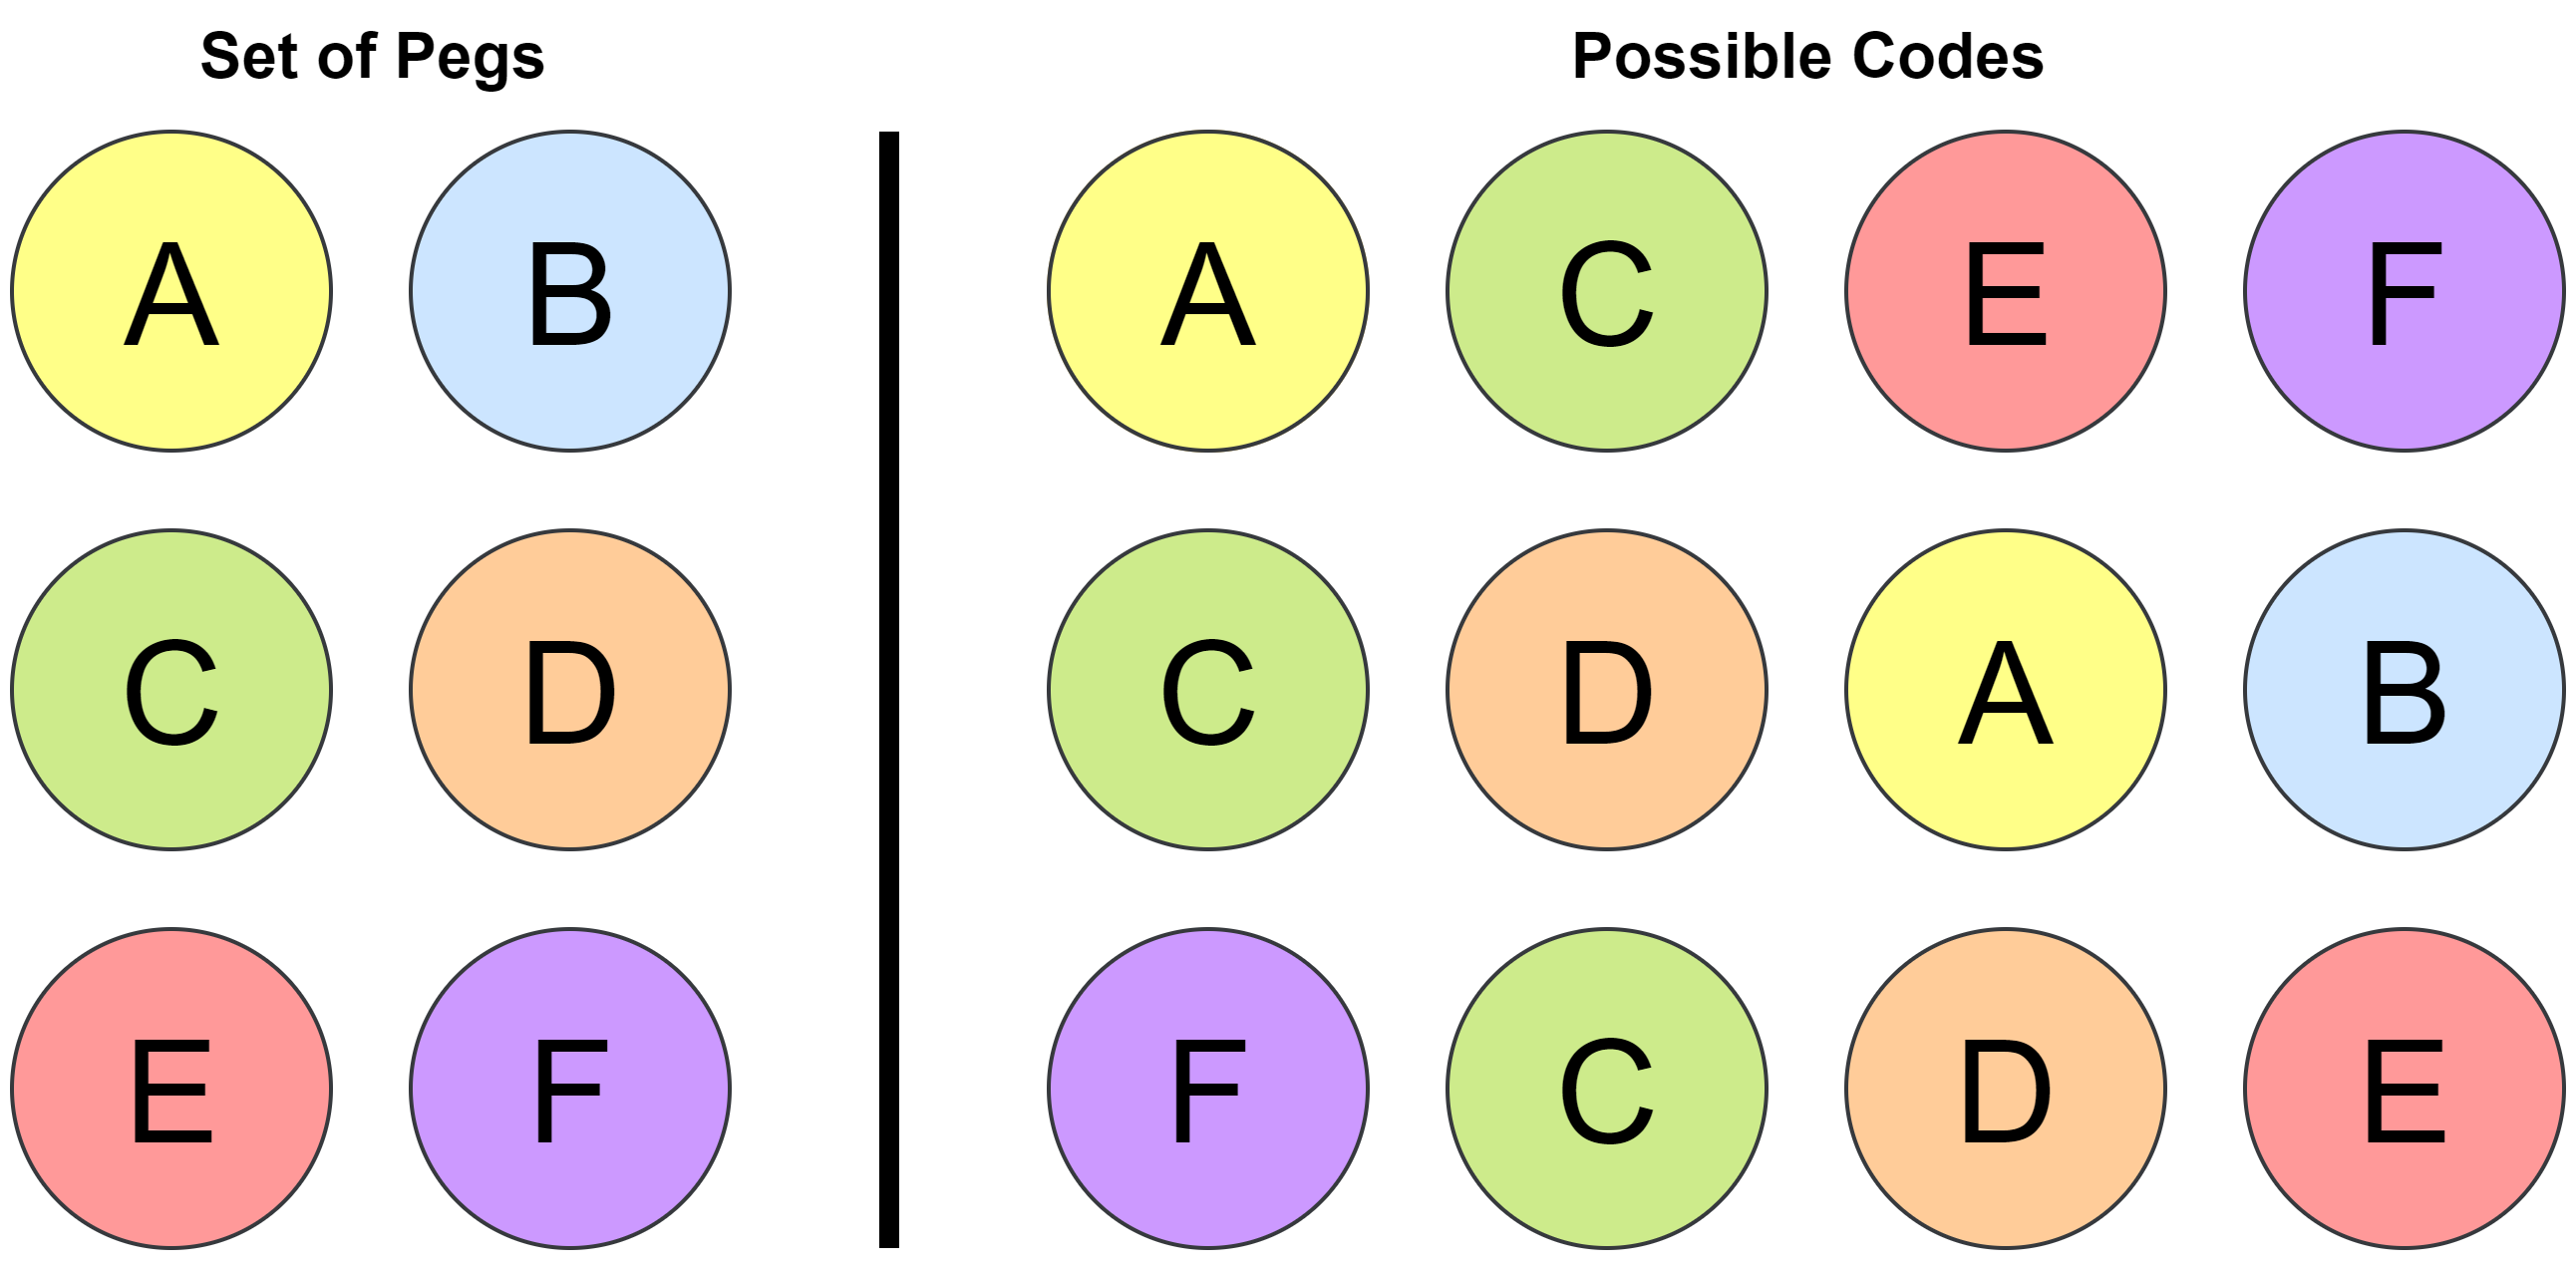
\includegraphics[scale=0.5]{pegs}
\caption{ Example codes which would satisfy the constraints of the standard variant of Mastermind.}
\end{figure}

The game begins once the secret code combination has been selected. The process of breaking the secret code consists of one player attempting a sequence of guesses as to the position and colours of the pegs in the code. Each attempt is followed by a hint which informs the player of how accurate their guess was in relation to the secret code. These hints inform the player if a correct colour was played in an incorrect position, most commonly represented with a white peg, and if a correct colour was played in a correct position, represented with a black peg.

\begin{figure}[H]
\centering
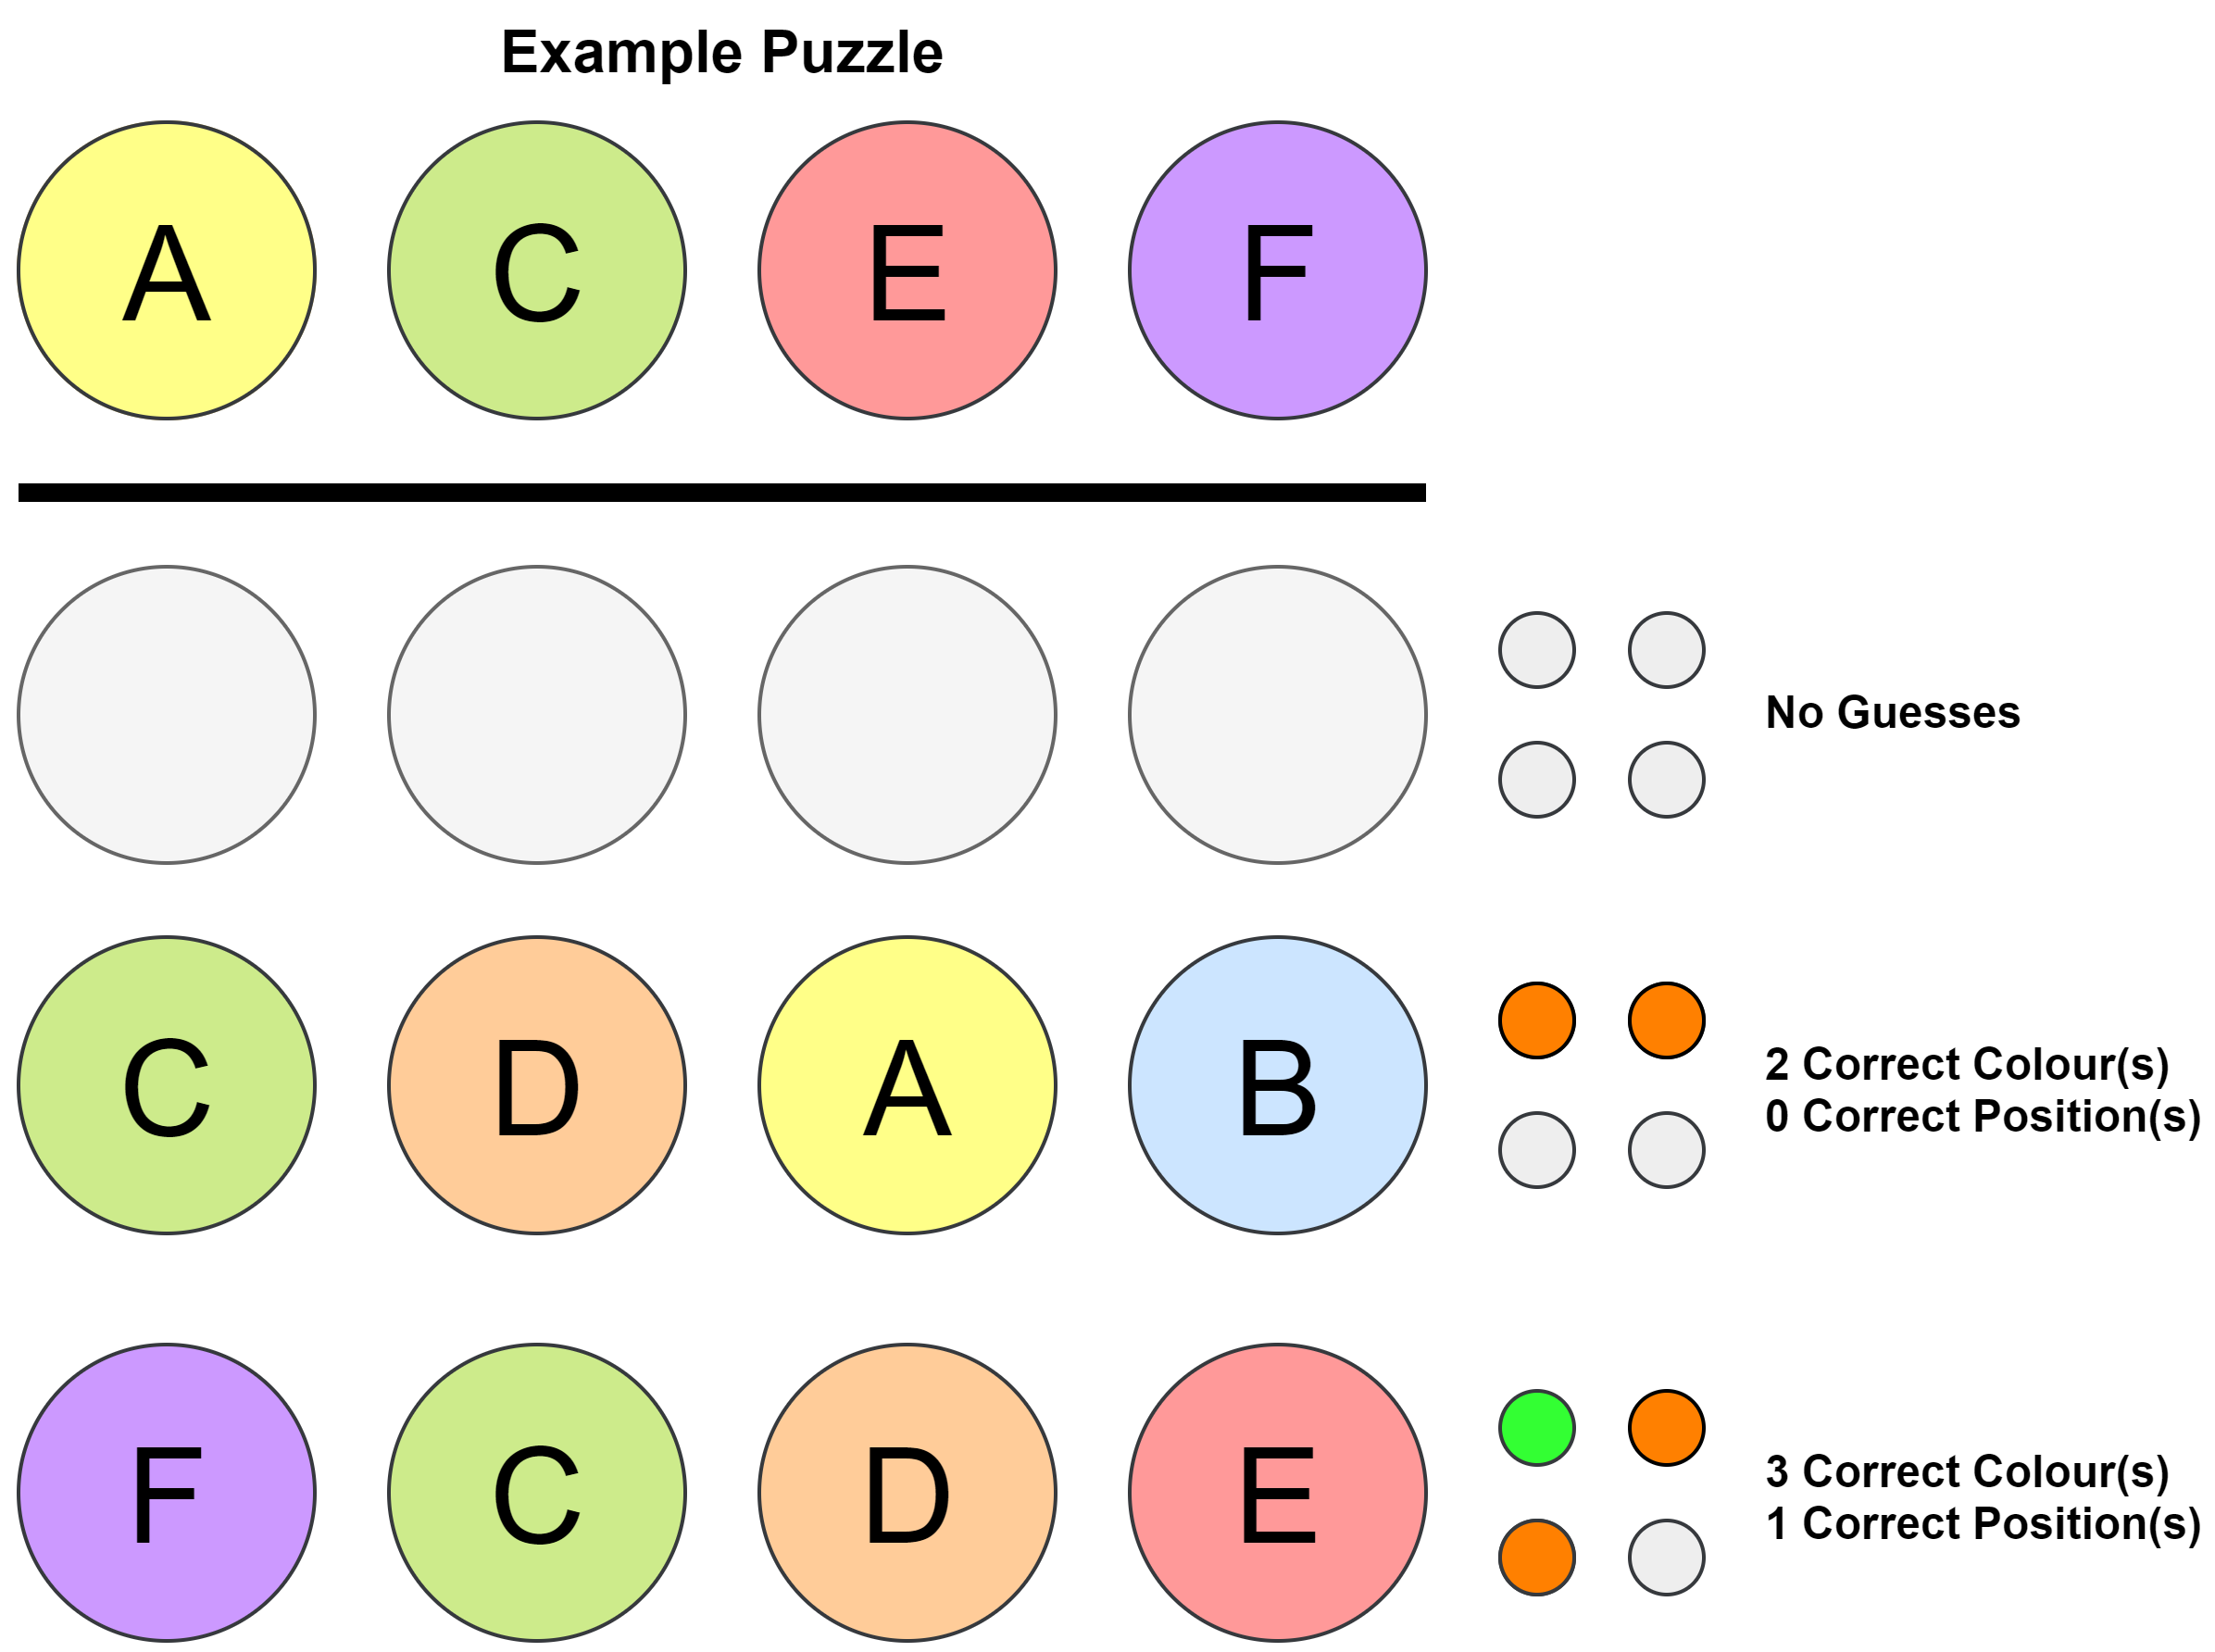
\includegraphics[scale=0.5]{guesses}
\caption{A simplified representation of a game state. The black and white hint pegs replaced with green and amber for clarity.}
\end{figure}

The game concludes when the correct code combination is discovered, represented through the hint system as four black pegs, or if a limit of guesses would be exceeded.

\subsubsection {Variations and Similar Problems}

Multiple variations of the original Mastermind game exist, most commonly varying either the length of the secret code, the size of the set of elements a code can be constructed from or both. One such example of this is the Super Mastermind variant which increments the code length to five elements and increases the possible elements to eight \cite {SuperMM}. These alterations result in 32 768 possible code combinations which could be selected as the secret code, a substantial increase over the 1 296 combinations of the standard variant. This increase becomes relevant when attempting to implement solutions to the puzzle as searching for a correct code combination in the larger sets poses challenges in time and memory \cite {ExhaustiveMM}.

\subsection {Problem Description and Fundamental Concepts}

\subsubsection {The Goal of a Solution}
To the perspective of the codebreaker Mastermind presents itself as a search problem which examines a set of all possible combinations which satisfy the given constraints and tasks the player with identifying the secret code within the set. An effective solution to Mastermind would be one that is able to traverse this set of all possible combinations and identify the secret code combination within it.

\subsubsection {Consistency and Search Strategies}

The search space associated with the standard variant of Mastermind contains 1,296 members, a naive strategy for finding the correct code amongst the collection could evaluation each entry individually to find a match to the secret code. A strategy which can prove efficient for smaller search spaces but is not viable as the size of the collection increases \cite{Two Peg}.

Previous Mastermind solutions would introduce a concept which would allow for easier traversal of these larger search spaces in the form of consistency. The logic behind this concept is that when an attempt is made to find the secret code combination the remaining search space that needs to be evaluated in later attempts is reduced due to that combination no longer being relevant to search and the hint provided from the attempt can deduce which combinations are incompatible with the secret code \cite {Merelo}. The consideration of a combination attempt and the resulting hint can be defined as a rule for that instance \cite {Haystack}. This can be shown for the example below:

\

Consider the secret code combination which represents the characters of the code as integers: '1111'. Prior to any search attempt the full range of 1,296 code combinations are equally probable to be the secret code. An attempt to evaluate the code '2332' returns a hint of zero white pegs and zero black pegs, informing the codebreaker that the symbols '2' and '3' do not appear in the secret code and therefore are not consistent with this instance. The only remaining possible code combinations are required to be consistent with this information, this forms the consistent search space. The consistent search space for this example would include all possible code combinations excluding those which contain either symbol '2' or '3'.

The concept of a consistent search space provides the basis for two categories of Mastermind solutions \cite{Haystack}:

\textbullet\ Stepwise Optimal: This strategy only selects code combinations which are consistent with the past attempts as defined previously. This method results in less combinations requiring evaluation due to redundant examples being ignored.

\textbullet\ Strategically Optimal: This strategy selects code combinations which allow for information relating to the appearance of the secret code to be deduced. The aim of a strategically optimal search strategy is to reduce the consistent search space by attempting suboptimal code combinations which provide information on the shape of the secret code.

\subsubsection {Donald E. Knuth Implementation}

One of the earliest proposed solutions to the Mastermind puzzle was a paper by Donald E. Knuth in which the claim is made that it is possible in all cases to arrive at the correct code within five attempts \cite {Wolfram} \cite {Knuth}. The algorithm that Knuth proposes utilises a strategically optimal method which focuses on selecting the combination at each step which will result in the largest reduction of the consistent search space.

\justify{
An example of the strategically optimal method can be shown below using Knuth's algorith, the members of the code represented with the integer range 1, ..., 6.}
\\

{
\centering
\begin{tabular}{cccc}
No. of Guesses & Test Pattern &  Hits  & Possible Combinations \\
0 & no guess & N/A & 1296 \\
1 & 1122 &  WWW  &  16 \\
2 & 1213 &  BWW  &  4 \\
\end {tabular} \par 
} 

At the initial point where no guess had been made the search space is still composed of all 1296 possible code combinations. This space of possible combinations is restricted using the result of the first guess which states that three of the chosen symbols were correct however their positions were incorrect. This information allows a great amount of restriction to only 16 possible code combinations which the code could belong to. The second guess restricts this space even further to just four possible combinations. Through this method Knuth asserted that it should be possible to achieve a correct guess within five test patterns. The starting pattern discovered by Knuth to give proof to this claim was found to be 1122. A possible progression of stages from this initial test pattern would be:
Another example is as follows:
\\

{
\centering
\begin{tabular}{cccc}
No. of Guesses & Test Pattern &  Hits  & Possible Combinations \\
0 & no guess & N/A & 1296 \\
1 & 1122 &  B  &  256 \\
2 & 1344 &  W  &  44 \\
1 & 3526 &  W  &  7 \\
\end {tabular} \par 
}

This situation would also allow for the next test pattern to distinguish the final possible combinations using the test pattern 1462. The algorithm places a high value on test patterns which coax the process towards the fourth guess being able to distinguish between the possible combinations. This method of solving the problem however is admitted within the paper to not be the most optimal solution. This can be shown by the way that the algorithm processes the following situation:
\\

{
\centering
\begin{tabular}{cccc}
No. of Guesses & Test Pattern &  Hits  & Possible Combinations \\
0 & no guess & N/A & 1296 \\
1 & 1122 &  BWW  &  16 \\
2 & 1213 &  BB  &  4 \\
\end {tabular} \par 
} 

which results in a possible four remaining code words (2212, 4212, 5212, 6212). The algorithm would select the test pattern 1145 as the next guess however when compared to the test pattern 4222 it can be shown that it in actuality results in less distinguishing results:
\\

{
\centering
\begin{tabular}{ccc}
Test Pattern          & Hits & Code  \\ \hline
\multirow{4}{*}{4222} & BWW  & 2212  \\
                      & BBB  & 4212  \\
                      & BB   & 5212  \\
                      & BB   & 62122 \\ \hline
\multirow{4}{*}{1145} & W    & 2212  \\
                      & WW   & 4212  \\
                      & WW   & 5212  \\
                      & W    & 62122
\end{tabular} \par
} 

It is clear that should 4222 be used at the test pattern there are two possibilities in 2212 and 4212 where the code can be known by the third guess. This is a better result compared to the test pattern 1145 where two possibilities will always be the result.

The advantage of using a search strategy such as the one that Knuth proposes is that because it is known in advance how the algorithm will behave for a set on inputs there is a gaurantee on the solution being found in a fixed number of attempts. The concession that is made with this confirmation of a fixed number of attempts however is that the algorithm may make suboptimal attempts due to the fixed path of how it evaluates the code combinations. This flaw leaves opportunities for other search strategies to surpass it in the amount of attempts required to arrive at a solution \cite {Haystack}.

\subsubsection {Risks in Searching}

RANDOMIZED SEARCH

\subsection {Progression of Solutions}

\subsubsection {Exhaustive Solutions}

\subsubsection {Evolutionary Computing}
A trend in modern solutions to Mastermind is the exploration of evolutionary computation as a tool for developing the algorithms which evaluate the best next step at each stage. 
This was the basis of research for the 2005 GenMM (Genetic Mastermind) algorithm which sought to compete with the exhaustive search implementations which were currently being investigated at that time [1]. 

Evolutionary computing serves as an adequate route for tackling decision problems such as the evaluation of possible steps to take whilst traversing the search space. 
The most common way this area is implemented is through the use of Evolutionary Algorithms which simulate the Darwinian natural evolution process to incrementally change the heuristics of a system [2].

\subsubsection {State of the Art}

%%% Where is progress currently
% Donald Knuth's implementation
% Exhaustive Solutions - Most Parts, Entropy, plus & plus2

\subsection {Functional Programming as a Tool}

\subsubsection {Functional Pearls}
The inspiration for this project was a paper by Richard Bird which implemented a solution to the puzzle game Sudoku as an example of a series of problems known as functional pearls. This section will explore the topic of functional pearls and their relevance to the current project. Functional Pearls begin as small problems which programmers wish to explore, focusing on brief but engaging examples that showcase either a guided explanation to a proof or presentation of unique data structures. The goal of a functional pearl is to teach important programming techniques and fundamental design principles \cite{Pearls}. Richard Bird described functional pearls in a speech as 'elegant, instructive examples of functional programming' while showcasing his implementation of a sudoku solution\cite {R. Bird Speech}.


The solution which this project aims to explore would enter the scope of a functional pearl due to its aim to document an example of functional programming. The project would however deviate from a traditional functional pearl as the scope would be expanded to consider similar solutions in the problem space to evaluate the different methods of solving Mastermind.

The functional pearl which inspired the project is Richard Birds paper 'Functional Pearl: A Program to Solve Sudoku' \cite{Sudoku}. The aim of the solution was to define the function:

\[ Sudoku :: Board \rightarrow [Board]\]

This function would take an input in the form of a Sudoku board, represented by a matrix of characters, and output a list of possible completed boards. Following this declaration the paper would proceed to use logic and equational reasoning to define the function using the functional language haskell to achieve the solution. Finally Richard Bird was able to arrive at the following definition for his solution:

\[ Sudoku :: Board \rightarrow [Board]\]
\[ Sudoku = map (map head) \bullet search \bullet prune \bullet choices\]

where search, prune and choices representing functions declared earlier in the implementation. These sudoku solutions provide an example of how the mastermind solution this project aims to implement may be approached. Aiming for a solution that resembles this process of declaring an initial function or set of functions then deriving a definition for them that can be evaluated through comparison with similar solutions. The next section will examine the problem that this project will aim to solve and the work that has been explored in the area previously.

\subsection {Applications Beyond Mastermind}

\subsubsection {Mastermind Complexity Class}
Mastermind belongs to a class of problems known as NP-Complete decision problems. This means that they are solvable in exponential time. A solution to Mastermind in polynomial time
would be an incredibly valuable resource as it would be proof that P = NP. This meaning that for all problems in class NP which are verifiable in polynomial time there exists a polynomial
solution to the problem. It is currently not known if this hypothesis that P = NP is true however it would be a great benefit to computer science as it would allow for problems such as
protein folding to be solved however it would also mean that encryption, a security method which relies on P != NP, would be rendered obsolete.

\newpage                     % optional page break
\section{Research Methodology and Requirements Analysis}\label{ss:back}

The base goal of this project is t

The scope of a Mastermind solution should focus on the combinatorial problem of how the search space, the set of all possible combinations, should be traversed. As has been explored in the background material the ability to navigate the possible combinations and the hints derived is integral to evaluating the correct steps to take to minimise the distance to a combination which matches the secret code. The research methodologies described in this chapter will propose several questions that this project hopes to answer through its implementation of a unique solution to the Mastermind puzzle. In support of these questions the requirements of the system which will be used to explore the research methodology will also be described.

\subsection {Research Methodology}

\subsubsection {Research Questions}

The scope of this project's investigations are broad due to the many differing approaches that have previously been explored. By defining a set of research questions the process of developing a solution can be structured around the aims and objectives stated at the beginning of this report. The research questions are as follows:

\

\textbf{1. How do exhaustive solutions to traversing the search space of a combinatorial problem compare to evolutionary methods?}

How can the scoring used in evolutionary search algorithms be improved in the context of ranking possible code combinations in the puzzle Mastermind.

Does sampling a population of possible solutions in a search space negatively effect the accuracy of the resulting algorithm when accounting for scale.

\

A large body of past work has focused on the applications of evolutionary computation, specifically genetic algorithms, to evaluate the combinations within the search space. The results of these implementations have been shown to have an advantage over previous solutions, some of which utilised an exhaustive approach which analysed each member of the search space. This inquiry provides a foundation for the base case of a solution, the results of which can be used as a metric for the evaluation of possible improvements in later iterations.

\

\textbf{2. What are the important factors to be considered when selecting the optimal combination from a search space?}

When approaching a large set of elements it is important to understand why a specific element from that set may be selected over another. The concept of consistency was introduced in the background material of this project which leads to the core of this question which asks how should this specific implementation evaluate which combination to select at each step. There already exists some work in this area presently such as the approach of partitioning combinations based on the hints provided through each guess, a starting step investigating this question can explore implementations utilising this method.

\

\textbf{3. What are the advantages of using functional programming as the basis for a solution to combinatorial search problems?}

\

If the implementation derived from this project is able to return a positive development in finding a solution to the Mastermind puzzle it should be noted to what extent the specific paradigm of functional programming is able to provide support. Following from this it can be investigated if the unique behaviours of functional programming provide benefits which would lend itself to being the optimal tool for further research into the area.
\subsection {Requirements Analysis}

\subsubsection {MoSCoW Prioritisation}

Description of the moscow prioritisation system.

\subsubsection {Functional Requirements}

The system must be capable of storing a list to represent the search space.
The system must be capable of storing a list to represent the consistent search space.
The system must be able to assign values to the elements of the consistent search space according to a fitness function.
The system must be able to iterate over the elements of the search space and consistent search space.
The system must be able to rank the elements of the consistent search space.

The system should allow for more than one size of search space.

\begin{tabularx}{\textwidth}{|X|X|X|}
\hline
ID     & Description                                                                         & Priority \\ \hline
FR 1.1 & The system must be capable of storing an integer combination of a given length.     & Must     \\ \hline
FR 1.2 & The system must be capable of generating an integer combination from a range of given integers and of a given length. & Must \\ \hline
FR 1.3 & The system must be capable of evaluating equality between two integer combinations. & Must     \\ \hline
FR 1.4 & The system must be capable of returning information on the similarity of a given input to the stored combination.     & Must \\ \hline
\end{tabularx}



\subsubsection {Non-Functional Requirements}

\newpage                     % optional page break
\section{Evaluation Strategy}\label{ss:back}

\subsection {Defining Metrics}

The evaluation of the solutions implemented in this project relate strongly to the research questions that we have defined in the previous section. Following from this means that the metrics on which our solutions will be evaluated on are as such:
\begin {itemize}
	\item {A solution which is able to restrict the consistent combination search space is considered more valuable.}
	\item {A solution which is more accurate in selecting the correct code from the consistent search space is more valuable.}
	\item {A solution which is able to scale elegantly with both an increase in possible symbols which comprise the code and an increase in the length of the code.}
\end{itemize}

\newpage
\section {Preliminary Work: The Base Solution}

\subsection {Design of a Base Solution}

\subsection {Results and Analysis of Base Solution}
In here talk about the work done with the current base solution. It will be originally done based on the donald knuth implementation.


\newpage                     % optional page break
\section{Project Management}\label{ss:back}

\subsection {Agile}

Description of the agile methodology and its advantages as it pertains to this project

\subsection {Gantt Chart}

The organisation of this project is represented by the following Gantt Chart, by utilising this chart the progress of later stages can be tracked and adjusted if there is a risk to the schedule.

\

[NEED TO FINISH THE GANTT FIGURE

\

It is important that each major milestone of the project is followed by a brief review period. The reason for this is to examine the schedule and provide mitigation measures if required.

\subsection {Risk Analysis and Mitigations}

\subsubsection {Risk Definitions}
To manage the progress of this project efficiently it was important to identify possible risks that could prevent the realisation of the goals laid out earlier in this document. To aid in the identification of the risks the following key was used to classify the associated risks:
\begin{itemize}
\item{People (P) - Risks which are the result of issues related to those individuals involved in the project. This relates to the wellbeing, scheduling and personal issues that can be encountered.}
\item{Technological (T) - Risks which can result from the technology being used to engineer the solutions. This relates to the technological constraints that could be encountered or the hardware required.}
\item{Requirement (R)  - Risks which can result from changes to the requirements of the project. This relates to problems encountered with the work being implemented for the project. Logical problems and issues with the material involved would be included in these risks.}
\end{itemize}

\begin{tabularx}{1.1\textwidth} {
	|  >{\center\arraybackslash}X
	| >{\center\arraybackslash}X
	| >{\center\arraybackslash}X
	| >{\center\arraybackslash} X | }
	\hline
	ID & Risk & Description \\
	\hline
	P/T/R1 & Textual Title of Risk & Textual Description of the Risk \\
	\hline
\end{tabularx}

\subsubsection {Risk Identification}

\begin{tabularx}{1.1\textwidth} {
	|  >{\center\arraybackslash}X
	| >{\center\arraybackslash}X
	| >{\center\arraybackslash}X
	| >{\center\arraybackslash} X | }
	\hline
	ID & Risk & Description \\
	\hline
	P.1 & Illness and Health Complications & The situation in which an individual involved in the project is unable to contribute due to illness or health complications. This risk is slightly heightened as the world recovers from the effects of the Covid-19 pandemic however it also considers other conditions which would require time away from the project. \\
	\hline
	T.1 & File Loss & This is the situation in which files or documents relating to the project are lost. This is a low priority issue as precautions have been taken to mitigate this such as using version control through Github. \\
	\hline
	R.1 & Insufficient Base Solution & The success of this project is dependent on having a solid base solution. The success of the base solution is assessed by a set of conditions which deems it suitable for solving the problem. The base solution being unable to meet these conditions is a serious situation and as such should be of a high priority. \\
	\hline
\end{tabularx}

\subsubsection {Risk Mitigation Procedures}

\subsection {Considerations of Professional, Legal, Ethical, and Social Issues}



%%%%%%%%%%%%%%%%%%%%%%%%%%%%%%%%%%%%%%%%%
%
%     Bibliography
%
%     Use an easy-to-remember tag for each entry - eg \bibitem{How97} for an article/book by Howie in 1997
%     To cite this publication in your text, write \cite{How97}.  To include more details such as
%     page, Chapter, Theorem numbers, use the form \cite[Theorem 6.3, page 42]{How97}.
%
\begin{thebibliography}{99}

% 
% The usual convention for mathematical bibliographies is to list alphabetically
% by first-named author (then second, third  etc. author then date)
% websites with no author names should go by the site name
%

% Typical layout for reference to a journal article
%\bibitem{Bovey}
%J. D. Bovey, M. M. Dodson,                         % author(s)
%The Hausdorff dimension of systems of linear forms % article name
%{\em Acta Arithmetica}                             % journal name - italics
%{\bf 45}                                           % volume number - bold
%(1986), 337--358.                                   % (year), page range


% Typical layout for reference to a book
%
%\bibitem{Cassels}
%J. W. S. Cassels,                                  % author(s)
%{\em An Introduction to Diophantine Approximation},% title - italics
%Cambridge University Press, Cambridge, 1965.       % Publisher, place, date.

% Typical layout for reference to a website
%
%\bibitem{GAP}
%The GAP Group, GAP -- Groups, Algorithms, and Programming,  % Site name
%Version 4.5.6; 2012. % other information
%(http://www.gap-system.org)  % URL


% Typical layout for reference to an online article

%\bibitem{Howie}
%J. Howie,                                            % author(s)
%{\em Generalised triangle groups of type $(3,5,2)$}, % article name - italics
%http://arxiv.org/abs/1102.2073                       % URL
%(2011).                                              % (year)

\bibitem {Wordle}
New York Times,
{\em "Wordle."}
https://www.nytimes.com/games/wordle/index.html
(Online, accessed 21-11-2022)

\bibitem {Wolfram}
Weisstein, Eric W.
{\em '"Mastermind." From Mathworld -- A Wolfram Web Resource.'}
https://mathworld.wolfram.com/Mastermind.html
(Online; accessed \today)

\bibitem {Invicta}
Invicta Toys and Games ltd.
{\em 'History of Mastermind.'}
https://web.archive.org/web/20070812104420/http://dspace.dial.pipex.com/town/road/gbd76/toys.htm
(Archived 2007)

\bibitem {Better Solutions}
J.-J. Merelo and T. P. Runarsson,
Finding Better Solutions to the Mastermind Puzzle Using Evolutionary Algorithms.
{\em 'Applications of Evolutionary Computing.'}
{\bf vol 6024}
(2010), pp 121-130

\bibitem {SuperMM}
Noble Knight Games,
{\em 'Super Master Mind - Boardgame from Invicta Games.'}
https://www.nobleknight.com/P/2147590038/Super-MasterMind
(Online; accessed \today)

\bibitem {ExhaustiveMM}
Merelo, J.J., Mora, A.M., Cotta, C. and Runarsson, T.P. 
{\em  ‘An experimental study of exhaustive solutions for the Mastermind puzzle.'}
(2012)
 doi:10.48550/arxiv.1207.1315.

\bibitem {Nelson}
Nelson, Toby.
{\em 'Investigations into the MasterMind Board Game'}
https://web.archive.org/web/20150906043015/http://www.tnelson.demon.co.uk/mastermind/index.html
(1999, Archived 2015)

\bibitem {Haystack}
Merelo-Guervós, J.J., Castillo, P. and Rivas, V.M. 
{\em ‘Finding a needle in a haystack using hints and evolutionary computation: the case of evolutionary MasterMind’, Applied soft computing}
{\bf  6(2)}
(2006) pp. 170–179. 
doi:10.1016/j.asoc.2004.09.003.

\bibitem {Two Peg}
Jäger, G.
An Optimal Strategy for Static Black-Peg Mastermind with Two Pegs.
{\em 'Combinatorial Optimization and Applications.'}
{\bf vol 10043}
(2016), pp 670–682
https://doi.org/10.1007/978-3-319-48749-6\_48

\bibitem {Knuth}
Knuth, Donald E. 
{\em 'The Computer as Master Mind', Recreational Mathematics}
{\bf 9(1)}
Stanford University
(1976, Baywood Publishing Co., Inc.)

\bibitem {Merelo}
 Merelo, J.J., Mora, A.M., Cotta, C. and Runarsson, T.P. 
{\em ‘An experimental study of exhaustive solutions for the Mastermind puzzle’.}
(2012) 

\bibitem {Pearls}
Bird, Richard.
{\em How to Write a Functional Pearl}
International Conference on Functional Programming, Portland
(2006)

\bibitem {R. Bird Speech}
Gibbons, Jeremy.
{\em University of Oxford, Functional Pearls}
http://www.cs.ox.ac.uk/people/jeremy.gibbons/pearls/
(2009)

\bibitem {Sudoku}
Bird, Richard.
{\em Functional Pearl, A Program to Solve Sudoku}
Cambridge University Press, Cambridge, 2006

\end{thebibliography}
\end{document}
